\section{Useful Memory and Temporal-Validity Horizons}
\label{sec:useful_memory_under_drift}

\begin{figure}[!htbp]
\centering
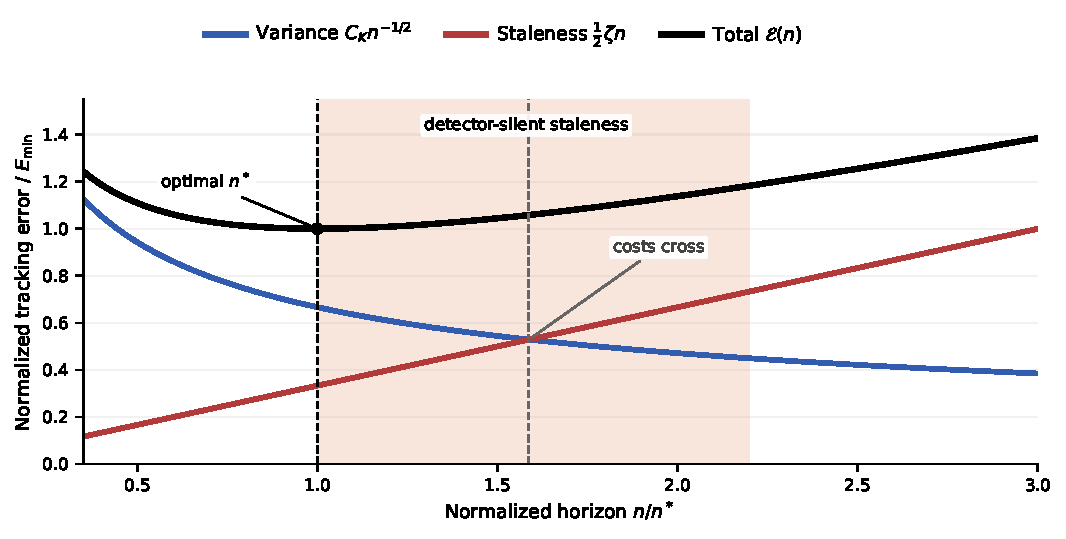
\includegraphics[width=0.92\linewidth]{artifacts/figures/conceptual/fig_two_clocks_of_drift.pdf}
\caption{Finite-sample--staleness trade-off under drift. The finite-sample term
falls with horizon, the staleness term rises with age, and total error is
minimized at the temporal-validity horizon $n^*$. The green band marks a
near-optimal useful-memory region, and the red band marks pre-detection
validity loss: retained evidence can stop representing the present before
enough changepoint evidence accumulates to trigger an alarm.}
\label{fig:finite_sample_staleness_tradeoff}
\end{figure}

For a finite-memory estimator with lag weights $w_0,\dots,w_{n-1}$, the natural
age variable is the effective lag
\[
  A(w) \coloneqq \sum_{j=0}^{n-1} j\,w_j.
\]
Its corresponding staleness at time $t$ is the weighted transport misalignment
\[
  S_t(w) \coloneqq \sum_{j=0}^{n-1} w_j\,
  W_2\!\left(P_{t-j},P_t\right).
\]
For a uniform window, $A(w)=(n-1)/2$, so window length and temporal age are the
same object up to constants.

Non-uniform weights separate two summaries. The finite-sample term is governed by
the effective sample size
\[
  n_{\mathrm{eff}}(w) \coloneqq \Bigl(\sum_{j=0}^{n-1} w_j^2\Bigr)^{-1},
\]
while the drift term is governed by weighted lag moments. For each $H\in(0,1]$,
define
\[
  M_H(w) \coloneqq \sum_{j=0}^{n-1} j^H w_j.
\]
Then any weighted horizon law of the form
\[
  \mathbb E\,d\!\left(\widehat P_t^{(w)},P_t\right)
  \le C_K n_{\mathrm{eff}}(w)^{-a} + C_S\zeta M_H(w)
\]
induces a weighted useful-memory region by balancing the two summaries. On a
linear ramp, $M_1(w)=A(w)$ exactly, so the effective lag recovers the exact
staleness term.

\begin{proposition}[Uniform weights maximize effective sample size]
\label{prop:uniform_maximizes_effective_sample_size}
Let $w_0,\dots,w_{n-1}$ be nonnegative weights with $\sum_{j=0}^{n-1} w_j=1$.
Then
\[
  n_{\mathrm{eff}}(w) \le n,
\]
with equality if and only if $w_j=1/n$ for all $j$. Moreover, if the drift
profile is an exact linear ramp in the sense that the lag-$j$ contribution is
proportional to $j$, then the weighted staleness equals the effective lag:
\[
  S_t(w)=c\,A(w)
\]
for the corresponding linear coefficient $c$.
\end{proposition}

\begin{proof}
By Cauchy--Schwarz,
\[
  1=\Bigl(\sum_{j=0}^{n-1} w_j\Bigr)^2
  \le n\sum_{j=0}^{n-1} w_j^2,
\]
so $n_{\mathrm{eff}}(w)=1/\sum_j w_j^2\le n$, with equality exactly when the
weights are all equal. On an exact linear ramp, the lag-$j$ contribution is
proportional to $j$, so averaging with weights $w_j$ gives the weighted mean lag
$A(w)$ and hence $S_t(w)=cA(w)$.
\end{proof}

Throughout, $P_t$ denotes the present target law,
$\bar P_t^{(n)}$ the window target obtained by averaging the last $n$ target
laws, and $\widehat P_t^{(n)}$ the estimator built from the last $n$
observations. The finite-sample term always refers to the estimation error
relative to $\bar P_t^{(n)}$, while the staleness term refers to the
discrepancy between $\bar P_t^{(n)}$ and $P_t$.

Finite-sample error relative to $\bar P_t^{(n)}$ and staleness relative to
$P_t$ combine into a horizon law. When both sides are controlled, the same scale
induces a useful-memory region: the range of memory lengths whose tracking
error remains near optimal.

\subsection{General Horizon Law}\label{subsec:abstract_upper_law}

The main theorem separates finite-sample behavior from drift-induced staleness.

\begin{theorem}[Abstract upper law]\label{thm:abstract_upper_law}
Let $d$ be a probability metric satisfying the triangle inequality. At time $t$,
let $P_t$ be the present target law, let $\bar P_t^{(n)}$ be the window target,
and let $\widehat P_t^{(n)}$ be the estimator built from the last $n$
observations. Assume that for some constants $C_K>0$, $C_S>0$, exponent $a>0$,
roughness index $H\in(0,1]$, and amplitude $\zeta>0$,
\[
  \mathbb E\,d\!\left(\widehat P_t^{(n)},\bar P_t^{(n)}\right)
  \le C_K n^{-a}
\]
and
\[
  d\!\left(\bar P_t^{(n)},P_t\right)
  \le C_S\zeta n^H
\]
hold for all $n$ in the regime of interest. Then
\[
  \mathbb E\,d\!\left(\widehat P_t^{(n)},P_t\right)
  \le C_K n^{-a} + C_S\zeta n^H.
\]
\end{theorem}

\begin{proof}
By the triangle inequality,
\[
  d\!\left(\widehat P_t^{(n)},P_t\right)
  \le
  d\!\left(\widehat P_t^{(n)},\bar P_t^{(n)}\right)
  + d\!\left(\bar P_t^{(n)},P_t\right).
\]
Taking expectations and applying the two assumptions yields the claim.
\end{proof}

The theorem isolates the structure of the problem:
the path class supplies the staleness term, while the chosen geometry and sample
regime supply the finite-sample term.

\begin{proposition}[Triangular-array transfer for Hadamard-differentiable functionals]
\label{prop:hadamard_triangular_transfer}
Let $\mathcal T$ be a functional on probability laws that is Hadamard
differentiable at $P_t$ tangentially to a linear subspace of signed measures, with
derivative $\dot{\mathcal T}_{P_t}$ bounded on the relevant tangent class. Suppose
that for the triangular-array estimator and its window target, the base metric
satisfies
\[
  \mathbb E\,d\!\left(\widehat P_t^{(n)},\bar P_t^{(n)}\right) \le C_K n^{-a}
\]
and the drift envelope satisfies
\[
  d\!\left(\bar P_t^{(n)},P_t\right) \le C_S\zeta n^H.
\]
If the remainder in the Hadamard expansion is $o(n^{-a})$ uniformly on the
relevant class, then there exist constants $\widetilde C_K,\widetilde C_S>0$
such that
\[
  \mathbb E\,\bigl\|\mathcal T(\widehat P_t^{(n)})-\mathcal T(P_t)\bigr\|
  \le \widetilde C_K n^{-a} + \widetilde C_S\zeta n^H.
\]
\end{proposition}

\begin{proof}
Write the Hadamard expansion at $P_t$ and apply the boundedness of the derivative
to the centered triangular-array fluctuation. The drift term contributes through
the same envelope as the base metric because $\mathcal T$ is locally Lipschitz on
the class. The remainder is lower order by assumption, so the transformed law
inherits the same horizon envelope.
\end{proof}

\begin{proposition}[Finite-dimensional smooth transfer]
\label{prop:smooth_finite_dimensional_transfer}
Let $\phi_1,\dots,\phi_k$ be bounded measurable functions and let
$Z(P)=\bigl(\mathbb E_P[\phi_1],\dots,\mathbb E_P[\phi_k]\bigr)$. Let
$g\in C^2(U)$ on an open set $U\subset\mathbb R^k$ containing the relevant
range of $Z$. Define $T(P)=g(Z(P))$. Suppose that on the triangular-array window
target and estimator,
\[
  \mathbb E\,\|Z(\widehat P_t^{(n)})-Z(\bar P_t^{(n)})\| \le C_K n^{-a}
\]
and
\[
  \|Z(\bar P_t^{(n)})-Z(P_t)\| \le C_S\zeta n^H.
\]
If the Hessian of $g$ is bounded by $M$ on the relevant range, then
\[
  \mathbb E\,|T(\widehat P_t^{(n)})-T(P_t)|
  \le \widetilde C_K n^{-a} + \widetilde C_S\zeta n^H,
\]
and the Taylor remainder is quadratic in the moment error:
\[
  \begin{aligned}
  |T(P')-T(P)-\nabla g(Z(P))^\top &\bigl(Z(P')-Z(P)\bigr)| \\
  \le \frac{M}{2}\|Z(P')-Z(P)\|^2.
  \end{aligned}
\]
\end{proposition}

\begin{proof}
Apply the multivariate Taylor formula to $g$ around $Z(P_t)$. The bounded Hessian
gives the stated quadratic remainder. The first-order term is controlled by the
assumed finite-sample and drift envelopes for $Z$, and the same decomposition as
in \cref{prop:hadamard_triangular_transfer} yields the horizon law for $T$.
\end{proof}

The same decomposition extends to non-uniform weights once the two summaries
$n_{\mathrm{eff}}(w)$ and $M_H(w)$ are controlled. The theorem-level question is
whether weighted forgetting enlarges the useful-memory region beyond a constant
factor on richer path classes, or whether it only changes the leading constant.

\begin{corollary}[Temporal-validity horizon]
\label{cor:temporal_validity_horizon}
Under the assumptions of \cref{thm:abstract_upper_law}, the upper envelope
\[
  \Phi(n) \coloneqq C_K n^{-a} + C_S\zeta n^H
\]
is minimized, up to constant factors depending only on $a$, $H$, and $C_S$, at
\[
  n^*(a,H) \asymp (C_K/\zeta)^{1/(a+H)},
\]
and the corresponding error scale is
\[
  \Phi(n^*) \asymp C_K^{H/(a+H)}\zeta^{a/(a+H)}.
\]
\end{corollary}

\begin{proof}
Balance the decreasing finite-sample term against the increasing staleness term:
\[
  C_K n^{-a} \asymp C_S\zeta n^H.
\]
This gives $n^{a+H}\asymp C_K/\zeta$, hence the displayed horizon law. Substituting
that scale back into either term gives the optimal error scale.
\end{proof}

Write the continuous optimizer of $\Phi$ as
\[
  n_\star \coloneqq \left(\frac{aC_K}{H C_S\zeta}\right)^{1/(a+H)}.
\]
This optimizer differs from the scale $n^*(a,H)$ only by constants depending on
$a$, $H$, and $C_S$, so the asymptotic horizon law remains unchanged.

\subsection{Useful-Memory Region}

The horizon scale induces a near-optimal region of memory lengths. For any
$\delta>0$, define the useful-memory region by
\[
  \mathcal U_\delta \coloneqq \{n>0: \Phi(n) \le (1+\delta)\Phi(n_\star)\}.
\]
This object records not only where the envelope is minimized, but also how much
memory remains acceptable up to a fixed tolerance.

\begin{proposition}[Useful-memory region at tolerance $\delta$]
\label{prop:useful_memory_region}
Let $\Phi(n)=C_K n^{-a}+C_S\zeta n^H$ with $a,H>0$, and let $n_\star$ be its
continuous optimizer. Then the normalized profile
\[
  \Psi(x) \coloneqq \frac{\Phi(n_\star x)}{\Phi(n_\star)}
  = \frac{H x^{-a} + a x^H}{a+H}
\]
is strictly decreasing on $(0,1]$ and strictly increasing on $[1,\infty)$.
Consequently,
\[
  \mathcal U_\delta = [n_-,n_+] = n_\star[x_-(\delta;a,H),x_+(\delta;a,H)],
\]
where $x_-(\delta;a,H)\le 1 \le x_+(\delta;a,H)$ are the two solutions of
$\Psi(x)=1+\delta$. In particular, the useful-memory region scales linearly with
the horizon scale $n_\star$, and its relative shape depends only on $a$, $H$,
and $\delta$.
\end{proposition}

\begin{proof}
Since $n_\star$ minimizes $\Phi$, differentiation gives
\[
  a C_K n_\star^{-a} = H C_S\zeta n_\star^H.
\]
Substituting $n=n_\star x$ into $\Phi$ and dividing by $\Phi(n_\star)$ yields
the displayed identity for $\Psi$. Differentiation then gives
\[
  \Psi'(x)=\frac{aH}{a+H}\bigl(x^{H-1}-x^{-a-1}\bigr),
\]
which is negative for $x<1$ and positive for $x>1$. Since $\Psi(1)=1$ and
$\Psi(x)\to\infty$ as $x\to 0$ or $x\to\infty$, the sublevel set
$\{x>0:\Psi(x)\le 1+\delta\}$ is a compact interval containing $1$, which
proves the representation of $\mathcal U_\delta$.
\end{proof}

For small tolerance, the useful-memory region has the local expansion
\[
  x_\pm(\delta;a,H) = 1 \pm \sqrt{\frac{2\delta}{aH}} + o(\sqrt{\delta}),
  \qquad \delta \downarrow 0,
\]
because $\Psi''(1)=aH$. The local curvature therefore controls how quickly the
near-optimal region contracts around the horizon.

The horizon depends jointly on the finite-sample rate exponent and the
roughness exponent. Different geometries and different drift regularities induce
different memory scales.

\subsection{Drift Regularity and Staleness Accumulation}

The staleness side of the law is controlled by a deterministic path class. For
$H\in(0,1]$ and $\zeta>0$, write
\[
  \mathfrak P_H(\zeta)
  \coloneqq
  \left\{(P_s)_{s\in\mathbb Z}: W_2(P_{t-j},P_t) \le \zeta j^H
  \text{ for all } j\ge 0\right\}.
\]
The case $H=1$ is the local Lipschitz envelope; smaller $H$ correspond to slower
accumulation of staleness with lag.

\begin{lemma}[Hölder staleness bound via averaged couplings]
\label{lem:Hölder_staleness_bound}
Let
\[
  \bar P_t^{(n)} \coloneqq \frac{1}{n}\sum_{j=0}^{n-1} P_{t-j}.
\]
If the target path belongs to $\mathfrak P_H(\zeta)$, then
\[
  W_2^2\!\left(\bar P_t^{(n)},P_t\right)
  \le
  \frac{\zeta^2}{n}\sum_{j=0}^{n-1} j^{2H},
\]
and therefore, by Jensen's inequality,
\[
  W_2\!\left(\bar P_t^{(n)},P_t\right)
  \le \zeta\left(\frac{1}{n}\sum_{j=0}^{n-1} j^{2H}\right)^{1/2}
  = C_{H,n}\,\zeta n^H,
\]
where
\[
  C_{H,n}
  \coloneqq
  \left(n^{-(2H+1)}\sum_{j=0}^{n-1} j^{2H}\right)^{1/2}.
\]
In particular, $C_{H,n}\to (2H+1)^{-1/2}$ as $n\to\infty$.
\end{lemma}

\begin{proof}
For each lag $j$, let $\pi_j$ be an optimal coupling between $P_{t-j}$ and $P_t$.
Their average
\[
  \bar \pi \coloneqq \frac{1}{n}\sum_{j=0}^{n-1} \pi_j
\]
couples $\bar P_t^{(n)}$ with $P_t$, so
\[
  \begin{aligned}
  W_2^2\!\left(\bar P_t^{(n)},P_t\right)
  &\le \int \|x-y\|^2\,d\bar\pi(x,y) \\
  &= \frac{1}{n}\sum_{j=0}^{n-1} W_2^2\!\left(P_{t-j},P_t\right).
  \end{aligned}
\]
Applying the Hölder envelope gives the displayed finite-$n$ constant, and taking
square roots completes the proof.
\end{proof}

Combining \cref{lem:Hölder_staleness_bound} with
\cref{cor:temporal_validity_horizon} yields the horizon family
\[
  n^*(a,H) \asymp (C_K/\zeta)^{1/(a+H)}.
\]
In the root-$n$ finite-sample regime $a=1/2$,
\[
  n^*(1/2,H) \asymp (C_K/\zeta)^{2/(1+2H)}.
\]
The finite-$n$ constant in
\cref{lem:Hölder_staleness_bound} is the constant used here for
uniform windows; the simpler $(2H+1)^{-1/2}$ expression is its large-window
limit.

\subsection{One-Dimensional Proof Model for the Root-$n$ Regime}
\label{subsec:one_dimensional_proof_model}

The bounded-support fixed-span one-dimensional triangular array provides a
tractable rigorous finite-sample instantiation of the abstract law. The model is
built on common compact support, uniformly regular window mixtures, and an
integrated Bahadur remainder hypothesis.

\begin{proposition}[Root-$n$ finite-sample bound in the 1D proof model]\label{prop:one_dimensional_root_n_bound}
Let $X_{n,1},\dots,X_{n,n}$ be independent one-dimensional observations with laws
$P_{n,1},\dots,P_{n,n}$, and define the window mixture
\[
  \bar P_n = \frac{1}{n}\sum_{j=1}^n P_{n,j}.
\]
Assume:
\begin{enumerate}[label=(\roman*)]
  \item all $P_{n,j}$ are supported on a common compact interval $[L,U]$;
  \item the within-window drift span is uniformly bounded in $n$;
  \item each mixture law $\bar P_n$ has a density $\bar f_n$ on $[L,U]$ that is
  bounded below by a positive constant and uniformly Hölder;
  \item writing $q_n$ for the quantile function of $\bar P_n$ and $\widehat q_n$
  for the empirical quantile function of $\widehat P_n^{\mathrm{tri}}$, one has
  the Bahadur representation
  \[
    \begin{aligned}
    \widehat q_n(u)-q_n(u)
    &= \frac{u-\widehat F_n(q_n(u))}{\bar f_n(q_n(u))} + R_n(u), \\
    &\hspace{2.2cm} u\in(0,1),
    \end{aligned}
  \]
  with
  \[
    \mathbb E\int_0^1 R_n(u)^2\,du=o(n^{-1}).
  \]
\end{enumerate}
Then
\[
  \mathbb E\,W_2^2\!\left(\widehat P_n^{\mathrm{tri}},\bar P_n\right)=O(n^{-1}),
\]
and therefore, by Jensen's inequality,
\[
  \mathbb E\,W_2\!\left(\widehat P_n^{\mathrm{tri}},\bar P_n\right)=O(n^{-1/2}).
\]
\end{proposition}

\begin{proof}
In one dimension,
\[
  W_2^2\!\left(\widehat P_n^{\mathrm{tri}},\bar P_n\right)
  = \int_0^1 \bigl(\widehat q_n(u)-q_n(u)\bigr)^2\,du,
\]
so the problem reduces to the integrated $L_2$ error of the empirical quantile
process. By item~(iv),
\[
  \widehat q_n(u)-q_n(u)
  =
  \frac{u-\widehat F_n(q_n(u))}{\bar f_n(q_n(u))} + R_n(u).
\]
Define
\[
  Z_n(u)\coloneqq \frac{u-\widehat F_n(q_n(u))}{\bar f_n(q_n(u))}.
\]
Then
\[
  \mathbb E\int_0^1 \bigl(\widehat q_n(u)-q_n(u)\bigr)^2du
  =
  \mathbb E\int_0^1 \bigl(Z_n(u)+R_n(u)\bigr)^2du.
\]
Let $m>0$ be a uniform lower bound for $\bar f_n$. Since
\[
  \widehat F_n(x)=\frac1n\sum_{j=1}^n \mathbf 1\{X_{n,j}\le x\},
\]
independence across the row gives
\[
  \operatorname{Var}(\widehat F_n(q_n(u)))
  =
  \frac{1}{n^2}\sum_{j=1}^n p_{n,j}(u)(1-p_{n,j}(u))
  \le \frac{1}{4n},
\]
where $p_{n,j}(u)=P_{n,j}(({-}\infty,q_n(u)])$. Therefore
\[
  \mathbb E\int_0^1 Z_n(u)^2du
  \le
  m^{-2}\int_0^1 \operatorname{Var}(\widehat F_n(q_n(u)))du
  \le \frac{1}{4m^2 n}.
\]
By item~(iv),
\[
  \mathbb E\int_0^1 R_n(u)^2du=o(n^{-1}).
\]
The cross term is then $o(n^{-1})$ by Cauchy--Schwarz, since
\(
  \mathbb E\int_0^1 Z_n(u)^2du=O(n^{-1})
\)
and
\(
  \mathbb E\int_0^1 R_n(u)^2du=o(n^{-1})
\).
Hence the expected squared Wasserstein error is $O(n^{-1})$, and Jensen's
inequality gives the root-$n$ rate for
$\mathbb E\,W_2\!\left(\widehat P_n^{\mathrm{tri}},\bar P_n\right)$.

The main conclusion is the exponent. Under this bounded-support fixed-span
regime, the triangular-array finite-sample term remains root-$n$.
\end{proof}

\subsection{Verifiable Sufficient Conditions for the 1D Proof Model}

An explicit deformation class makes the proof-model hypotheses verifiable. Let
\[
  g_\delta(x)=x+\delta x(1-x), \qquad x\in[0,1], \qquad |\delta|\le \Delta<1.
\]
Then $g_\delta$ is an increasing $C^2$ diffeomorphism of $[0,1]$, with
\[
  1-\Delta \le g_\delta'(x) \le 1+\Delta, \qquad |g_\delta''(x)|\le 2\Delta,
\]
so the transformed densities satisfy
\[
  \frac{1}{1+\Delta}\le f_\delta(y) \le \frac{1}{1-\Delta},
\]
and the same support is preserved.

\begin{corollary}[Verifiable Bahadur remainder for the smooth deformation class]
\label{cor:bahadur_sufficient_conditions_smooth_deformation}
Assume that each row law has the form
\[
  P_{n,j}=(g_{\delta_{n,j}})_\#\,\mathrm{Unif}[0,1],
  \qquad |\delta_{n,j}|\le \Delta<1,
\]
and that the within-window span is uniformly bounded in $n$. Then item~(iv) of
\cref{prop:one_dimensional_root_n_bound} holds. More precisely, there exists a
constant $C_\Delta<\infty$ such that
\[
  \mathbb E\int_0^1 R_n(u)^2\,du \le C_\Delta n^{-2}.
\]
Consequently,
\[
  \mathbb E\,W_2\!\left(\widehat P_n^{\mathrm{tri}},\bar P_n\right)=O(n^{-1/2})
\]
on this deformation class.
\end{corollary}

\begin{proof}
Write $\bar F_n$ and $q_n$ for the mixture cdf and quantile. Since each
$g_{\delta_{n,j}}$ is an increasing diffeomorphism of $[0,1]$, every mixture law
$\bar P_n$ is supported on $[0,1]$ and has density
$\bar f_n=\frac1n\sum_{j=1}^n f_{\delta_{n,j}}$ satisfying the explicit bounds
\[
  \frac{1}{1+\Delta}\le \bar f_n(y)\le \frac{1}{1-\Delta},
  \qquad
  \|\bar f_n'\|_\infty\le \frac{2\Delta}{(1-\Delta)^3}.
\]
Hence the inverse map $\bar F_n^{-1}$ is uniformly twice differentiable on
$(0,1)$, with second derivative bounded by a constant depending only on
$\Delta$. Applying the second-order Taylor expansion of $\bar F_n^{-1}$ around
$u=\bar F_n(q_n(u))$ gives
\[
  \widehat q_n(u)-q_n(u)
  = \frac{u-\widehat F_n(q_n(u))}{\bar f_n(q_n(u))} + R_n(u),
\]
with
\[
  |R_n(u)|\le C_\Delta\,|\widehat F_n(q_n(u))-u|^2.
\]
Now
\[
  \widehat F_n(q_n(u))
  =\frac1n\sum_{j=1}^n \mathbf 1\{X_{n,j}\le q_n(u)\}
\]
is an average of independent Bernoulli variables with mean $u$. Uniformly in
$u$, its fourth centered moment is $O(n^{-2})$. Therefore
\[
  \mathbb E\,R_n(u)^2\le C_\Delta\,\mathbb E|\widehat F_n(q_n(u))-u|^4
  \le C_\Delta' n^{-2},
\]
and integrating over $u\in(0,1)$ yields
\[
  \mathbb E\int_0^1 R_n(u)^2\,du\le C_\Delta' n^{-2}=o(n^{-1}).
\]
The root-$n$ claim then follows from \cref{prop:one_dimensional_root_n_bound}.
The same smoothness package is consistent with the classical Bahadur theory of
\citet{Bahadur1966} and \citet[Chapter~21]{vanDerVaart1998}, but here the
explicit deformation bounds make the integrated remainder quantitative.
\end{proof}

\begin{remark}[Weak rowwise dependence]
The proof of \cref{prop:one_dimensional_root_n_bound} uses independence within a
row only through the $O(n^{-1})$ variance bound for the empirical cdf term and
through item~(iv). Consequently, the same root-$n$ conclusion persists under any
short-range dependent rowwise model for which the empirical cdf still has
$L_2$ fluctuation of order $n^{-1/2}$ and the integrated Bahadur remainder
remains $o(n^{-1})$. Short-range mixing conditions are one natural route to such
a package, but the present paper does not develop a general dependent-row
theorem.
\end{remark}

On the tested smooth fixed-support family, the integrated residual decays at
empirical rates between $1.40$ and $1.54$ for spans $0.2$ and $0.4$, and the
scaled quantity $n\int_0^1 R_n(u)^2du$ still decays at rates between $0.40$ and
$0.54$; see \cref{app:finite_sample_geometry}. On the fixed-span triangular-array
uniform-kernel model, the residual-to-MSE ratio drops from about $0.38$ at
$n=25$ to about $0.11$ at $n=400$, with integrated residual rates $1.43$ for the
triangular sample and $1.49$ for the i.i.d. mixture benchmark. These diagnostics
do not replace a general verification theorem, but they sit behind an
explicit sufficient-condition corollary on the smooth deformation class and
quantify span dependence on the tested classes.

\subsection{Structural Lower Bound in the Root-$n$ Regime}\label{subsec:lower_bound}

The upper law would be substantially weaker if it were only an estimator-specific
statement. The lower bound shows that, in the root-$n$ finite-sample regime
$a=1/2$, the horizon is imposed by the drift geometry itself.

\begin{figure}[!htbp]
\centering
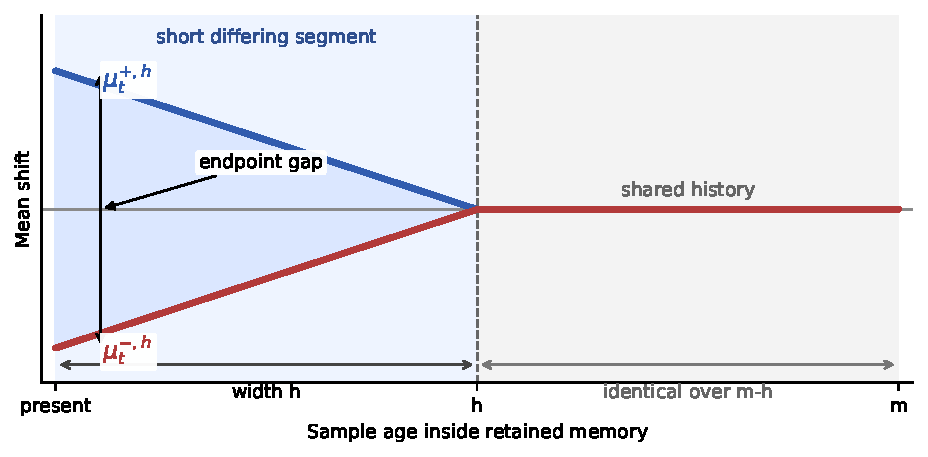
\includegraphics[width=0.88\linewidth]{artifacts/figures/conceptual/fig_lower_bound_witness.pdf}
\caption{Gaussian lower-bound construction. The two paths share
most of the retained history and differ only on a recent segment of width $h$,
yet remain separated at the present. That recent segment already produces the
same horizon exponent as the upper law in the root-$n$ regime.}
\label{fig:lower_bound_construction}
\end{figure}

\begin{proposition}[Structural lower bound in the root-$n$ regime]
\label{prop:structural_lower_bound}
Fix $H\in(0,1]$ and work on the Gaussian location subclass with known variance
$\sigma^2$ and path pair
\[
  \mu_{t-j}^{\pm,h} = \pm \beta (h-j)_+^H,
  \qquad j=0,1,\dots,h,
\]
where $\beta\le \zeta$ enforces the roughness budget. Let
$\mathcal G_{H,\zeta}^{\mathrm{Gauss}}$ denote the corresponding Gaussian
location subclass of target paths, and suppose the retained observations are
independent with laws $N(\mu_{t-j}^{\pm,h},\sigma^2)$. Then there exists a
constant $c_H>0$ depending only on $H$ such that the endpoint tracking risk over
this subclass satisfies
\[
  \inf_{\widehat P}\sup_{P\in\mathcal G_{H,\zeta}^{\mathrm{Gauss}}}
  \mathbb E\,W_2\!\left(\widehat P_t,P_t\right)
  \ge c_H\,\sigma^{2H/(2H+1)}\zeta^{1/(2H+1)}.
\]
Consequently, in the root-$n$ finite-sample regime $a=1/2$, the horizon scale
\[
  h^*(H) \asymp (\sigma/\zeta)^{2/(2H+1)}
\]
is structural even on this restricted subclass.
\end{proposition}

\paragraph{Proof.}
Compare two hypotheses generated by the path pair
$\mu_{t-j}^{+,h}$ and $\mu_{t-j}^{-,h}$. At the present time, the endpoint
separation is of order $\beta h^H$. On the Gaussian location subclass, this is
also the $W_2$ separation. The Kullback--Leibler divergence between the two
hypotheses is proportional to
\[
  \beta^2 \sum_{r=1}^h r^{2H}/\sigma^2.
\]
Choosing
\[
  \beta = \min\!\left\{\zeta,\frac{\sigma}{2\sqrt{\sum_{r=1}^h r^{2H}}}\right\}
\]
keeps the testing problem in the Le Cam regime while respecting the roughness
budget. The resulting two-point lower bound is of order $\beta h^H$. Balancing
the active roughness constraint against the testing constraint gives
$h^*(H)\asymp (\sigma/\zeta)^{2/(2H+1)}$ and therefore the displayed lower law.
The exact Gaussian two-point calculation used here is recorded in
\cref{app:proof_details}.

The lower bound is subclass based and not class-tight, but it is enough to show
that the horizon is a structural feature of the problem and not an estimator
artifact.

The proposition above is the lower-bound fact needed for the main horizon law.
The same Gaussian construction also exposes the constant-level geometry.
The following proposition records the sharp Gaussian constants available within
that proof scheme.

\subsection{Gaussian Lower-Bound Geometry}
\label{subsec:gaussian_lower_bound_geometry}

Let $\Phi$ and $\varphi$ denote the standard normal distribution function and
density.
\begin{proposition}[Gaussian lower-bound constants]
\label{prop:gaussian_lower_bound_constants}
Fix $H\in(0,1]$ and set $p_H \coloneqq 2H/(2H+1)$. Let $x_H>0$ be the unique
maximizer of $x^{p_H}\Phi(-x)$, equivalently the unique solution of
\[
  p_H\Phi(-x_H)=x_H\varphi(x_H).
\]
For the Gaussian ramp profile $\mu_{t-j}^{\pm,h}=\pm\zeta(h-j)_+^H$, let
\[
  L_h^{\mathrm{ramp}}(\sigma,\zeta)
  \coloneqq
  \zeta h^H\Phi\!\left(-\frac{\zeta}{\sigma}\sqrt{\sum_{r=1}^h r^{2H}}\right).
\]
Then, as $\sigma/\zeta\to\infty$,
\[
  \sup_{h\ge 1} L_h^{\mathrm{ramp}}(\sigma,\zeta)
  \sim
  C_H^{\mathrm{ramp}}\,\sigma^{2H/(2H+1)}\zeta^{1/(2H+1)},
\]
with
\[
  C_H^{\mathrm{ramp}}
  =
  (2H+1)^{H/(2H+1)}x_H^{2H/(2H+1)}\Phi(-x_H).
\]
Among all endpoint-saturating H\"older profiles, the profile
\[
  g_r^{\min}=h^H-(h-r)^H
\]
minimizes the testing energy and has asymptotic energy constant
\[
  I_H
  =
  \int_0^1 \left(1-(1-u)^H\right)^2du
  =
  \frac{2H^2}{(H+1)(2H+1)}.
\]
If
\[
  L_h^{\min}(\sigma,\zeta)
  \coloneqq
  \zeta h^H\Phi\!\left(-\frac{\zeta}{\sigma}\sqrt{\sum_{r=1}^h (g_r^{\min})^2}\right),
\]
then, as $\sigma/\zeta\to\infty$,
\[
  \sup_{h\ge 1} L_h^{\min}(\sigma,\zeta)
  \sim
  C_H^{\min}\,\sigma^{2H/(2H+1)}\zeta^{1/(2H+1)},
\]
with
\[
  C_H^{\min}
  =
  I_H^{-H/(2H+1)}x_H^{2H/(2H+1)}\Phi(-x_H).
\]
For $H<1$, this strictly improves the ramp constant by the factor
\[
  \frac{C_H^{\min}}{C_H^{\mathrm{ramp}}}
  =
  \left(\frac{H+1}{2H^2}\right)^{H/(2H+1)}
  >1,
\]
while at $H=1$ the two profiles coincide.
\end{proposition}

\begin{proof}
The exact Gaussian testing problem reduces the two-point lower bound to the
displayed quantities $L_h^{\mathrm{ramp}}$ and $L_h^{\min}$. After rescaling by
$h=A(\sigma/\zeta)^{2/(2H+1)}$, the ramp energy and endpoint-minimal energy have
limits $(2H+1)^{-1}$ and $I_H$, respectively. The corresponding normalized
payoff becomes a scalar multiple of $x^{p_H}\Phi(-x)$, whose unique maximizer is
$x_H$. The endpoint-minimal profile minimizes testing energy among all
endpoint-saturating H\"older profiles, so it yields the sharper constant. Full
details are given in \cref{app:proof_details}.
\end{proof}

These constants sharpen the lower-bound picture without changing the horizon
exponents or the status of the main results.

The same lower-bound geometry also yields a full class-level benchmark once
the model is specialized to Gaussian location tracking. In that setting, the
deterministic H\"older envelope, the finite-memory estimator, and the lower-bound
construction all live in the same one-dimensional parameterization, so this
model admits a direct minimax rate statement.

\begin{theorem}[Gaussian location minimax benchmark on the deterministic H\"older class]
\label{thm:gaussian_location_minimax_holder}
Fix $H\in(0,1]$, $\zeta>0$, and $\sigma>0$. Let $\mathfrak M_H(\zeta)$ denote the
class of deterministic mean paths $(\mu_s)_{s\in\mathbb Z}$ such that
\[
  |\mu_{t-j}-\mu_t|\le \zeta j^H
  \qquad\text{for all }j\ge 0.
\]
Suppose the observations are independent with
\[
  Y_{t-j}\sim N(\mu_{t-j},\sigma^2),
  \qquad j=0,1,\dots,n-1,
\]
and let the target law at time $t$ be $P_t=N(\mu_t,\sigma^2)$. Define the
optimal finite-memory minimax risk
\[
  \mathcal R_H^*(\sigma,\zeta)
  \coloneqq
  \inf_{n\ge 1}
  \inf_{\widehat P_t^{(n)}}
  \sup_{\mu\in\mathfrak M_H(\zeta)}
  \mathbb E\,W_2\!\left(\widehat P_t^{(n)},P_t\right).
\]
Then there exist constants $0<c_H\le C_H<\infty$, depending only on $H$, such
that
\[
  \begin{aligned}
  c_H\,\sigma^{2H/(2H+1)}\zeta^{1/(2H+1)}
  &\le \mathcal R_H^*(\sigma,\zeta) \\
  &\le C_H\,\sigma^{2H/(2H+1)}\zeta^{1/(2H+1)}.
  \end{aligned}
\]
In particular, the deterministic H\"older class has horizon scale
\[
  n_H^*\asymp (\sigma/\zeta)^{2/(2H+1)}.
\]
Moreover, the uniform-window mean estimator has an exact asymptotic upper
constant on this benchmark. If $y_H>0$ solves
\[
  H y_H\bigl(2\Phi(y_H)-1\bigr)=\varphi(y_H),
\]
then its asymptotic horizon shape is
\[
  A_H^{\mathrm{mean}}=((H+1)y_H)^{2/(2H+1)}
\]
and its asymptotic risk constant is
\[
  \begin{aligned}
  U_H^{\mathrm{mean}}
  &= ((H+1)y_H)^{-1/(2H+1)} \\
  &\quad \times \Bigl(2\varphi(y_H)+y_H\bigl(2\Phi(y_H)-1\bigr)\Bigr).
  \end{aligned}
\]
\end{theorem}

\begin{proof}
For the upper bound, estimate the present mean by the uniform-window average
\[
  \widehat\mu_t^{(n)}\coloneqq \frac{1}{n}\sum_{j=0}^{n-1}Y_{t-j}
\]
and set $\widehat P_t^{(n)}=N(\widehat\mu_t^{(n)},\sigma^2)$. Because equal-variance
Gaussian laws satisfy
\[
  W_2\!\left(N(m_1,\sigma^2),N(m_2,\sigma^2)\right)=|m_1-m_2|,
\]
the risk reduces to mean estimation error. The noise term is
$\sigma\sqrt{2/(\pi n)}$, while the deterministic bias is bounded by
\[
  \frac{\zeta}{n}\sum_{j=0}^{n-1} j^H,
\]
so
\[
  \sup_{\mu\in\mathfrak M_H(\zeta)}
  \mathbb E\,W_2\!\left(\widehat P_t^{(n)},P_t\right)
  \le
  \sigma\sqrt{\frac{2}{\pi n}} + \frac{\zeta}{n}\sum_{j=0}^{n-1} j^H.
\]
Rescaling by $n=A(\sigma/\zeta)^{2/(2H+1)}$ yields a one-parameter normalized
upper envelope. Differentiating its exact Gaussian-location form gives the stated
root equation for $y_H$, and therefore the displayed asymptotic upper constant
and horizon shape. In particular, this proves the stated upper rate and horizon
scale.

For the lower bound, use the symmetric two-point subfamily
\[
  \mu_{t-j}^{\pm,h}=\pm \beta\bigl(h^H-j^H\bigr)_+,
  \qquad j\ge 0,
\]
with $\beta\le \zeta$. This family lies in $\mathfrak M_H(\zeta)$ because
\[
  |\mu_t^{\pm,h}-\mu_{t-j}^{\pm,h}|=\beta\min(h^H,j^H)\le \zeta j^H.
\]
Moreover, for fixed endpoint value $\beta h^H$, it minimizes the Gaussian testing
energy over all symmetric lag profiles allowed by the present-point H\"older
envelope, since each lag coordinate is independently minimized by
$\beta(h^H-j^H)_+$. The exact Gaussian two-point calculation from the lower-bound
analysis in \cref{app:proof_details} therefore applies on the full deterministic H\"older class and
yields a lower bound of order
\[
  \sigma^{2H/(2H+1)}\zeta^{1/(2H+1)}.
\]
Minimizing over $h$ gives the same horizon scale $(\sigma/\zeta)^{2/(2H+1)}$.
Combining the two sides proves the theorem.
\end{proof}

\subsection{Multivariate Extension via Finite Projection Families, Sliced, and Product Geometries}

The horizon law also extends beyond one dimension when the multivariate geometry
reduces to a uniformly controlled family of one-dimensional transport problems.
This is the natural setting for sliced or coordinate-averaged Wasserstein
constructions, where the finite-sample term is built by integrating projected
one-dimensional errors.

\begin{corollary}[Finite-family projection transfer]\label{cor:finite_projection_transfer}
Let $\Pi=\{\theta_1,\dots,\theta_m\}$ be a finite family of linear maps from the
ambient space to $\mathbb R$, and define
\[
  d_{\Pi}(P,Q)
  \coloneqq
  \Bigl(\frac{1}{m}\sum_{r=1}^m
  W_2^2\!\left(P_{\theta_r},Q_{\theta_r}\right)\Bigr)^{1/2}.
\]
Assume that for every $r=1,\dots,m$:
\begin{enumerate}[label=(\roman*)]
  \item the projected triangular-array window satisfies the hypotheses of
  \cref{prop:one_dimensional_root_n_bound} with constants uniform in $r$;
  \item the projected drift path obeys the same H\"older staleness envelope with
  exponent $H$ and amplitude at most $\zeta$ uniformly in $r$.
\end{enumerate}
Then there exist constants $C_{K,\Pi},C_{S,\Pi}<\infty$ such that
\[
  \mathbb E\,d_{\Pi}\!\left(\widehat P_t^{(n)},P_t\right)
  \le C_{K,\Pi} n^{-1/2} + C_{S,\Pi}\zeta n^H.
\]
Consequently,
\[
  n_{\Pi}^*(H)\asymp (C_{K,\Pi}/\zeta)^{1/(H+1/2)}.
\]
In particular, the same law holds for coordinate-averaged product
constructions obtained by taking $\Pi$ to be the coordinate projections.
\end{corollary}

\begin{proof}
For each $r$, \cref{prop:one_dimensional_root_n_bound} gives
\[
  \mathbb E\,W_2^2\!\left(\widehat P_{t,\theta_r}^{(n)},\bar P_{t,\theta_r}^{(n)}\right)
  \le C n^{-1}
\]
with $C$ uniform in $r$. Averaging over $r$ yields
\[
  \mathbb E\,d_{\Pi}^2\!\left(\widehat P_t^{(n)},\bar P_t^{(n)}\right)
  \le C n^{-1},
\]
and Jensen gives the root-$n$ bound for
$\mathbb E\,d_{\Pi}(\widehat P_t^{(n)},\bar P_t^{(n)})$. The projected H\"older
bound averages in the same way:
\[
  d_{\Pi}\!\left(\bar P_t^{(n)},P_t\right)
  \le C_{S,\Pi}\zeta n^H.
\]
Applying \cref{thm:abstract_upper_law} with $d=d_{\Pi}$ yields the displayed
envelope and horizon scale.
\end{proof}

\begin{corollary}[Sliced-Wasserstein transfer under uniform projected control]
\label{cor:sliced_wasserstein_transfer}
Let $\rho$ be a probability measure on a family of one-dimensional projections
$\theta$, and define
\[
  SW_{2,\rho}^2(P,Q)
  \coloneqq \int W_2^2(P_{\theta},Q_{\theta})\,\rho(d\theta),
\]
where $P_{\theta}$ denotes the pushforward of $P$ under projection $\theta$.
Assume that for every $\theta$ in the support of $\rho$:
\begin{enumerate}[label=(\roman*)]
  \item the projected triangular-array window satisfies the hypotheses of
  \cref{prop:one_dimensional_root_n_bound} with constants uniform in $\theta$;
  \item the projected drift path obeys the same H\"older staleness envelope with
  exponent $H$ and amplitude at most $\zeta$ uniformly in $\theta$.
\end{enumerate}
Then there exist constants $C_K,C_S<\infty$ such that
\[
  \mathbb E\,SW_{2,\rho}\!\left(\widehat P_t^{(n)},P_t\right)
  \le C_K n^{-1/2} + C_S\zeta n^H.
\]
Consequently,
\[
  n^*(H)\asymp (C_K/\zeta)^{1/(H+1/2)}.
\]
Finite projection families are included by taking $\rho$ supported on finitely
many atoms; \cref{cor:finite_projection_transfer} states that case directly for
multivariate tracking.
\end{corollary}

\begin{proof}
For each projection $\theta$, \cref{prop:one_dimensional_root_n_bound} gives
\[
  \mathbb E\,W_2^2\!\left(\widehat P_{t,\theta}^{(n)},\bar P_{t,\theta}^{(n)}\right)
  \le C n^{-1}
\]
with $C$ uniform in $\theta$. Integrating over $\rho$ yields
\[
  \mathbb E\,SW_{2,\rho}^2\!\left(\widehat P_t^{(n)},\bar P_t^{(n)}\right)
  \le C n^{-1},
\]
and Jensen gives the root-$n$ bound for
$\mathbb E\,SW_{2,\rho}(\widehat P_t^{(n)},\bar P_t^{(n)})$. The projected
H\"older bound integrates in the same way, giving
\[
  SW_{2,\rho}\!\left(\bar P_t^{(n)},P_t\right)\le C_S\zeta n^H.
\]
Applying \cref{thm:abstract_upper_law} with $d=SW_{2,\rho}$ yields the stated
envelope and horizon scale.
\end{proof}

\subsection{Benchmark Theorems and Operational Extensions}

The Gaussian benchmark and the fixed-$\varepsilon$ Sinkhorn extension place the
horizon law in two broader settings: a full path-class benchmark with theorem-
level closure, and an operational transport geometry in which the one-
dimensional compact-support inheritance theory is already explicit. The
linear-Gaussian entropic-OT setting suggests an intermediate recursive regime
between the i.i.d. fixed-$\varepsilon$ theory and the embedded low-dimensional
extension \citep{Kalman1960,Jazwinski1970,AkyildizEtAl2024}.

\paragraph{Fixed-$\varepsilon$ Sinkhorn setting.}
For fixed-$\varepsilon$ debiased Sinkhorn, the central question is whether a
practical geometry can supply a stable finite-sample term on the embedded
fixed-span model. The target law is
\[
  \mathbb E\,S_{\varepsilon}\!\left(\widehat P_{t,\mathrm{tri}}^{(n)},\bar P_t^{(n)}\right)
  \le C_{\varepsilon} n^{-a_{\varepsilon}}
\]
under bounded support, fixed span, and structural low-dimensionality, where
$S_{\varepsilon}$ denotes a fixed-$\varepsilon$ Sinkhorn-type geometry and the
exponent $a_{\varepsilon}$ matches the corresponding i.i.d. mixture benchmark.

\begin{definition}[Fixed-$\varepsilon$ Sinkhorn setting]
\label{def:fixed_epsilon_sinkhorn_setting}
Fix a bounded embedded fixed-span model, an intrinsic complexity index $k$, a
dual H\"older smoothness level $\alpha$, and an operational band
$\mathcal B\subset(0,\infty)$ of regularization values. We say that this model
is in the fixed-$\varepsilon$ Sinkhorn setting if:
\begin{enumerate}[label=(\roman*)]
  \item the i.i.d. fixed-$\varepsilon$ benchmark on the same support class
  admits a finite-sample bound with exponent $a_{\varepsilon}$ on $\mathcal B$;
  \item the triangular-window and i.i.d.-mixture supports have identical
  operational covering complexity on $\mathcal B$;
  \item the dual class lies in the parametric adaptation region $\alpha>k/2$.
\end{enumerate}
\end{definition}

\begin{proposition}[Structural ingredients for fixed-$\varepsilon$ Sinkhorn]
\label{prop:operational_sinkhorn_ingredients}
On the bounded embedded fixed-span model with squared-Euclidean cost, the first
three items in \cref{def:fixed_epsilon_sinkhorn_setting} are structural: the
support-complexity inheritance is exact, and the dual-complexity condition is
precisely the LCA threshold $\alpha>k/2$.
\end{proposition}

\begin{proposition}[Conditional embedded moderate-band Sinkhorn inheritance]
\label{prop:conditional_embedded_sinkhorn_inheritance}
Fix the calibrated embedded fixed-span model with intrinsic dimension $k=2$ and
a compact moderate band $\mathcal B=[\varepsilon_{\min},\varepsilon_{\max}]$
bounded away from zero. Assume:
\begin{enumerate}[label=(\roman*)]
  \item a centered self-coupling stability lemma holds uniformly on $\mathcal B$
  with a spectral-radius bound strictly below one and a uniform inverse-norm
  bound on the centered subspace;
  \item the centered Sinkhorn scaling map admits a uniform implicit-function
  linearization on $\mathcal B$ with remainder $o(n^{-1/2})$;
  \item the induced influence class satisfies a root-$n$ triangular empirical-
  process bound on the embedded support class;
  \item the embedded fixed-span support and dual-complexity hypotheses of
  \cref{prop:operational_sinkhorn_ingredients} hold.
\end{enumerate}
Then there exists a finite constant $C_{\mathcal B}$ such that
\[
  \sup_{\varepsilon\in\mathcal B}
  \mathbb E\,S_{\varepsilon}\!
  \left(\widehat P_{t,\mathrm{tri}}^{(n)},\bar P_t^{(n)}\right)
  \le C_{\mathcal B} n^{-1/2}.
\]
Consequently the corresponding temporal-validity horizon on $S_{\varepsilon}$ has
the root-$n$ horizon scale
\[
  n^*_{\mathcal B}(H)
  \asymp
  \left(C_{\mathcal B}/\zeta\right)^{1/(H+1/2)}.
\]
\end{proposition}

\begin{proof}
Under (i)--(iii), the regularized Sinkhorn value admits a uniform first-order
expansion on $\mathcal B$ with a remainder lower order than $n^{-1/2}$. The
embedded fixed-span support and dual-complexity hypotheses in (iv) supply the
same structural comparison needed in the 1D proof model. Applying the abstract
horizon law with $a=1/2$ yields the stated envelope and the induced horizon
scale.
\end{proof}

\begin{proposition}[Pointwise fixed-$\varepsilon$ inheritance in the 1D proof model]
\label{prop:pointwise_sinkhorn_1d}
Assume the hypotheses of \cref{prop:one_dimensional_root_n_bound}, let
$\widehat P_n^{\mathrm{iid}}$ be the empirical measure of $n$ i.i.d. samples from
$\bar P_n$, and fix $\varepsilon>0$. For the debiased Sinkhorn divergence
$S_{\varepsilon}$ with squared-Euclidean cost on the common compact support,
one has
\[
  \mathbb E\,S_{\varepsilon}\!\left(\widehat P_n^{\mathrm{tri}},\bar P_n\right)
  = O(n^{-1/2}).
\]
\end{proposition}

\begin{proof}
Write $V_{\varepsilon}(\mu,\nu)$ for the regularized OT value so that
\[
  S_{\varepsilon}(\mu,\nu)
  = V_{\varepsilon}(\mu,\nu)
  - \tfrac12 V_{\varepsilon}(\mu,\mu)
  - \tfrac12 V_{\varepsilon}(\nu,\nu).
\]
Because all measures are supported on one compact interval, they lie in a
common bounded quadratic-moment class. By \citet[Thm.~3.7(ii), Ex.~3.4]{EcksteinNutz2022},
for fixed $\varepsilon$ there exists $L_{\varepsilon}<\infty$ depending only on
that class and on the cost such that
\[
  |V_{\varepsilon}(\mu,\nu)-V_{\varepsilon}(\mu',\nu')|
  \le L_{\varepsilon}\bigl(W_2(\mu,\mu')+W_2(\nu,\nu')\bigr).
\]
Applying this bound to the cross term and both self terms gives
\[
  |S_{\varepsilon}(\mu,\nu)-S_{\varepsilon}(\mu',\nu')|
  \le 2L_{\varepsilon}\bigl(W_2(\mu,\mu')+W_2(\nu,\nu')\bigr).
\]
With $\nu=\nu'=\bar P_n$,
\[
  S_{\varepsilon}\!\left(\widehat P_n^{\mathrm{tri}},\bar P_n\right)
  \le
  S_{\varepsilon}\!\left(\widehat P_n^{\mathrm{iid}},\bar P_n\right)
  + 2L_{\varepsilon}
    W_2\!\left(\widehat P_n^{\mathrm{tri}},\widehat P_n^{\mathrm{iid}}\right).
\]
Taking expectations and using the triangle inequality gives
\[
  \mathbb E\,W_2\!\left(\widehat P_n^{\mathrm{tri}},\widehat P_n^{\mathrm{iid}}\right)
  \le
  \mathbb E\,W_2\!\left(\widehat P_n^{\mathrm{tri}},\bar P_n\right)
  + \mathbb E\,W_2\!\left(\widehat P_n^{\mathrm{iid}},\bar P_n\right).
\]
The first term is $O(n^{-1/2})$ by \cref{prop:one_dimensional_root_n_bound}. The second is
the classical i.i.d. one-dimensional quantile-process rate on the same compact
support class \citep{Bahadur1966,vanDerVaart1998}, so it is also
$O(n^{-1/2})$. Hence
\[
  \mathbb E\,W_2\!\left(\widehat P_n^{\mathrm{tri}},\widehat P_n^{\mathrm{iid}}\right)
  = O(n^{-1/2}).
\]
Finally, under the null comparison with fixed $\varepsilon$ and compact support,
the i.i.d. debiased Sinkhorn term satisfies
\[
  \mathbb E\,S_{\varepsilon}\!\left(\widehat P_n^{\mathrm{iid}},\bar P_n\right)
  = O(n^{-1})
\]
by \citet[Thm.~5.1, after fixed-$\varepsilon$ rescaling]{delBarrioEtAl2023}; see also the null-limit law in
\citet{GoldfeldEtAl2022}. Combining the bounds yields the displayed
$O(n^{-1/2})$ rate.
\end{proof}

\begin{proposition}[Bandwise fixed-$\varepsilon$ inheritance in the 1D proof model]
\label{prop:bandwise_sinkhorn_1d}
Let $\mathcal B=[\varepsilon_{\min},\varepsilon_{\max}]\subset(0,\infty)$ be a
compact regularization band. Under the hypotheses of
\cref{prop:pointwise_sinkhorn_1d} on a common compact support class, there exists
$C_{\mathcal B}<\infty$ such that
\[
  \sup_{\varepsilon\in\mathcal B}
  \mathbb E\,S_{\varepsilon}\!\left(\widehat P_n^{\mathrm{tri}},\bar P_n\right)
  \le C_{\mathcal B} n^{-1/2}.
\]
Consequently, the induced horizon scale is uniform on $\mathcal B$:
\[
  \sup_{\varepsilon\in\mathcal B} n_{\varepsilon}^*(H)
  \asymp (C_{\mathcal B}/\zeta)^{1/(H+1/2)}.
\]
\end{proposition}

\begin{proof}
Repeat the proof of \cref{prop:pointwise_sinkhorn_1d}. The stability constant
$L_{\varepsilon}$ from \citet[Thm.~3.7(ii), Ex.~3.4]{EcksteinNutz2022} is bounded
on $\mathcal B$ because all measures live in one compact support class and
$\varepsilon\ge\varepsilon_{\min}>0$. The i.i.d. debiased-Sinkhorn benchmark on
compact support is also uniform on $\mathcal B$ by the fixed-$\varepsilon$
asymptotics of \citet{GoldfeldEtAl2022} and the compact-support null bounds of
\citet[Thm.~5.1, after fixed-$\varepsilon$ rescaling]{delBarrioEtAl2023}. Since
the triangular-to-i.i.d. $W_2$ comparison is independent of $\varepsilon$, the
  constants in the pointwise proof can be chosen uniformly over $\mathcal B$.
\end{proof}

\begin{proposition}[Conditional embedded fixed-$\varepsilon$ band inheritance]
\label{prop:conditional_embedded_sinkhorn_band}
Assume the fixed-$\varepsilon$ Sinkhorn setting from
\cref{def:fixed_epsilon_sinkhorn_setting}. Suppose that on a compact band
$\mathcal B=[\varepsilon_{\min},\varepsilon_{\max}]$, the centered Sinkhorn
scaling map admits a uniform linearization with remainder $o(n^{-1/2})$ and a
uniform self-coupling inverse bound. Then there exists $C_{\mathcal B}<\infty$
such that
\[
  \sup_{\varepsilon\in\mathcal B}
  \mathbb E\,S_{\varepsilon}\!\left(\widehat P_{t,\mathrm{tri}}^{(n)},\bar P_t^{(n)}\right)
  \le C_{\mathcal B} n^{-1/2}.
\]
Consequently, on any such band the induced horizon scale satisfies
\[
  \sup_{\varepsilon\in\mathcal B} n_{\varepsilon}^*(H)
  \asymp (C_{\mathcal B}/\zeta)^{1/(H+1/2)}.
\]
\end{proposition}

\begin{proof}
The linearization hypothesis reduces the triangular-array Sinkhorn divergence to
its first-order influence term plus an $o(n^{-1/2})$ remainder. The uniform
self-coupling inverse bound keeps the influence operator bounded across
$\mathcal B$, while the triangular-array fluctuation of the empirical measure is
root-$n$ on the embedded fixed-span class. The same balance then gives the
uniform $n^{-1/2}$ bound and the stated horizon scale.
\end{proof}

\begin{conjecture}[Bandwise fixed-$\varepsilon$ Sinkhorn horizon inheritance]
\label{conj:embedded_sinkhorn_horizon}
Beyond the one-dimensional fixed-$\varepsilon$ band result above, assume the fixed-$\varepsilon$ Sinkhorn setting from
\cref{def:fixed_epsilon_sinkhorn_setting}. Then, on bands where the i.i.d.
benchmark stays in the parametric Sinkhorn regime, the triangular-array
finite-sample term should satisfy
\[
  \mathbb E\,S_{\varepsilon}\!\left(\widehat P_{t,\mathrm{tri}}^{(n)},\bar P_t^{(n)}\right)
  \le C_{\varepsilon} n^{-1/2},
  \qquad \varepsilon\in\mathcal B,
\]
and the corresponding horizon scale should satisfy
\[
  n_{\varepsilon}^*(H) \asymp (C_{\varepsilon}/\zeta)^{1/(H+1/2)}.
\]
More generally, if the i.i.d. benchmark on $\mathcal B$ has exponent
$a_{\varepsilon}$, then the operational horizon law should be
\[
  n_{\varepsilon}^*(a_{\varepsilon},H)
  \asymp (C_{\varepsilon}/\zeta)^{1/(a_{\varepsilon}+H)}.
\]
\end{conjecture}

\paragraph{Evidence.}
The i.i.d. benchmark comes from existing fixed-$\varepsilon$ entropic transport
results, including fixed-marginal limit theory for the Sinkhorn divergence and
intrinsic-complexity adaptation \citep{GoldfeldEtAl2022,Stromme2023MID,
GroppeHundrieser2024LCA}. In the present embedded fixed-span model,
support-complexity inheritance is exact and the dual smoothness threshold
reduces to $\alpha>k/2$. Calibration then asks whether triangular and i.i.d.
rate estimates remain close across the regularization band. Additional
one-dimensional smooth fixed-support diagnostics show that triangular and i.i.d.
fitted exponents can agree closely on moderate fixed-$\varepsilon$ bands, while
direct Jacobian diagnostics concentrate the remaining difficulty on uniform
control of the self-coupling derivative blocks across nontrivial bands and
higher-dimensional embedded classes.

Regular dominated families remain the natural family-level extension class.
Local testing geometry and metric comparability suggest the same horizon logic
with a modified finite-sample exponent, whereas support-changing and singular
families fall outside that regime.

Once a finite-sample regime and a roughness level are specified, the law yields
an explicit memory scale and an optimal error scale. Rougher drift and weaker
finite-sample rates both force shorter memory and larger residual error.
